% Template for PLoS
% Version 3.5 March 2018
%
% % % % % % % % % % % % % % % % % % % % % %
%
% -- IMPORTANT NOTE
%
% This template contains comments intended 
% to minimize problems and delays during our production 
% process. Please follow the template instructions
% whenever possible.
%
% % % % % % % % % % % % % % % % % % % % % % % 
%
% Once your paper is accepted for publication, 
% PLEASE REMOVE ALL TRACKED CHANGES in this file 
% and leave only the final text of your manuscript. 
% PLOS recommends the use of latexdiff to track changes during review, as this will help to maintain a clean tex file.
% Visit https://www.ctan.org/pkg/latexdiff?lang=en for info or contact us at latex@plos.org.
%
%
% There are no restrictions on package use within the LaTeX files except that 
% no packages listed in the template may be deleted.
%
% Please do not include colors or graphics in the text.
%
% The manuscript LaTeX source should be contained within a single file (do not use \input, \externaldocument, or similar commands).
%
% % % % % % % % % % % % % % % % % % % % % % %
%
% -- FIGURES AND TABLES
%
% Please include tables/figure captions directly after the paragraph where they are first cited in the text.
%
% DO NOT INCLUDE GRAPHICS IN YOUR MANUSCRIPT
% - Figures should be uploaded separately from your manuscript file. 
% - Figures generated using LaTeX should be extracted and removed from the PDF before submission. 
% - Figures containing multiple panels/subfigures must be combined into one image file before submission.
% For figure citations, please use "Fig" instead of "Figure".
% See http://journals.plos.org/plosone/s/figures for PLOS figure guidelines.
%
% Tables should be cell-based and may not contain:
% - spacing/line breaks within cells to alter layout or alignment
% - do not nest tabular environments (no tabular environments within tabular environments)
% - no graphics or colored text (cell background color/shading OK)
% See http://journals.plos.org/plosone/s/tables for table guidelines.
%
% For tables that exceed the width of the text column, use the adjustwidth environment as illustrated in the example table in text below.
%
% % % % % % % % % % % % % % % % % % % % % % % %
%
% -- EQUATIONS, MATH SYMBOLS, SUBSCRIPTS, AND SUPERSCRIPTS
%
% IMPORTANT
% Below are a few tips to help format your equations and other special characters according to our specifications. For more tips to help reduce the possibility of formatting errors during conversion, please see our LaTeX guidelines at http://journals.plos.org/plosone/s/latex
%
% For inline equations, please be sure to include all portions of an equation in the math environment.  For example, x$^2$ is incorrect; this should be formatted as $x^2$ (or $\mathrm{x}^2$ if the romanized font is desired).
%
% Do not include text that is not math in the math environment. For example, CO2 should be written as CO\textsubscript{2} instead of CO$_2$.
%
% Please add line breaks to long display equations when possible in order to fit size of the column. 
%
% For inline equations, please do not include punctuation (commas, etc) within the math environment unless this is part of the equation.
%
% When adding superscript or subscripts outside of brackets/braces, please group using {}.  For example, change "[U(D,E,\gamma)]^2" to "{[U(D,E,\gamma)]}^2". 
%
% Do not use \cal for caligraphic font.  Instead, use \mathcal{}
%
% % % % % % % % % % % % % % % % % % % % % % % % 
%
% Please contact latex@plos.org with any questions.
%
% % % % % % % % % % % % % % % % % % % % % % % %

\documentclass[10pt,letterpaper]{article}
\usepackage[top=0.85in,left=2.75in,footskip=0.75in]{geometry}

% amsmath and amssymb packages, useful for mathematical formulas and symbols
\usepackage{amsmath,amssymb}

% Use adjustwidth environment to exceed column width (see example table in text)
\usepackage{changepage}

% Use Unicode characters when possible
\usepackage[utf8x]{inputenc}

% textcomp package and marvosym package for additional characters
\usepackage{textcomp,marvosym}

% cite package, to clean up citations in the main text. Do not remove.
\usepackage{cite}

% Use nameref to cite supporting information files (see Supporting Information section for more info)
\usepackage{nameref,hyperref}

% line numbers
\usepackage[right]{lineno}

% ligatures disabled
\usepackage{microtype}
\DisableLigatures[f]{encoding = *, family = * }

% color can be used to apply background shading to table cells only
\usepackage[table,dvipsnames]{xcolor}

% array package and thick rules for tables
\usepackage{array}

%strikethrough
\usepackage{soul}

%sara: for commenting the pdf to add alt text (if anyone knows a better solution for atl text please help)
\usepackage{pdfcomment}

% create "+" rule type for thick vertical lines
\newcolumntype{+}{!{\vrule width 2pt}}

% create \thickcline for thick horizontal lines of variable length
\newlength\savedwidth
\newcommand\thickcline[1]{%
  \noalign{\global\savedwidth\arrayrulewidth\global\arrayrulewidth 2pt}%
  \cline{#1}%
  \noalign{\vskip\arrayrulewidth}%
  \noalign{\global\arrayrulewidth\savedwidth}%
}

% \thickhline command for thick horizontal lines that span the table
\newcommand\thickhline{\noalign{\global\savedwidth\arrayrulewidth\global\arrayrulewidth 2pt}%
\hline
\noalign{\global\arrayrulewidth\savedwidth}}


% Remove comment for double spacing
%\usepackage{setspace} 
%\doublespacing

% Text layout
\raggedright
\setlength{\parindent}{0.5cm}
\textwidth 5.25in 
\textheight 8.75in

% Bold the 'Figure #' in the caption and separate it from the title/caption with a period
% Captions will be left justified
\usepackage[aboveskip=1pt,labelfont=bf,labelsep=period,justification=raggedright,singlelinecheck=off]{caption}
\renewcommand{\figurename}{Fig}

% Use the PLoS provided BiBTeX style
\bibliographystyle{plos2015}

% Remove brackets from numbering in List of References
\makeatletter
\renewcommand{\@biblabel}[1]{\quad#1.}
\makeatother



% Header and Footer with logo
\usepackage{lastpage,fancyhdr,graphicx}
\usepackage{epstopdf}
%\pagestyle{myheadings}
\pagestyle{fancy}
\fancyhf{}
%\setlength{\headheight}{27.023pt}
%\lhead{\includegraphics[width=2.0in]{PLOS-submission.eps}}
\rfoot{\thepage/\pageref{LastPage}}
\renewcommand{\headrulewidth}{0pt}
\renewcommand{\footrule}{\hrule height 2pt \vspace{2mm}}
\fancyheadoffset[L]{2.25in}
\fancyfootoffset[L]{2.25in}
\lfoot{\today}

%% Include all macros below

\newcommand{\lorem}{{\bf LOREM}}
\newcommand{\ipsum}{{\bf IPSUM}}

%% END MACROS SECTION


\begin{document}

\newcommand{\fede}[1]{\textcolor{ForestGreen}{Fede: #1}}
\newcommand{\rocio}[1]{\textcolor{MidnightBlue}{Rocio: #1}}
\newcommand{\doro}[1]{\textcolor{RedViolet}{Dorothea: #1}}
\newcommand{\jani}[1]{\textcolor{YellowOrange}{Janina: #1}}
\newcommand{\la}[1]{\textcolor{RawSienna}{Laura: #1}}

\vspace*{0.2in}

% Title must be 250 characters or less.
\begin{flushleft}
{\Large
\textbf\newline{Ten simple rules towards hosting an inclusive conference} % Please use "sentence case" for title and headings (capitalize only the first word in a title (or heading), the first word in a subtitle (or subheading), and any proper nouns).
}
\newline
% Insert author names, affiliations and corresponding author email (do not include titles, positions, or degrees).
\\
Name1 Surname\textsuperscript{1,2\Yinyang},
Name2 Surname\textsuperscript{2\Yinyang},
Name3 Surname\textsuperscript{2,3\textcurrency},
Name4 Surname\textsuperscript{2},
Name5 Surname\textsuperscript{2\ddag},
Name6 Surname\textsuperscript{2\ddag},
Name7 Surname\textsuperscript{1,2,3*},
with the Lorem Ipsum Consortium\textsuperscript{\textpilcrow}
\\
\bigskip
\textbf{1} Affiliation Dept/Program/Center, Institution Name, City, State, Country
\\
\textbf{2} Affiliation Dept/Program/Center, Institution Name, City, State, Country
\\
\textbf{3} Affiliation Dept/Program/Center, Institution Name, City, State, Country
\\
\bigskip

% Insert additional author notes using the symbols described below. Insert symbol callouts after author names as necessary.
% 
% Remove or comment out the author notes below if they aren't used.
%
% Primary Equal Contribution Note
\Yinyang These authors contributed equally to this work.

% Additional Equal Contribution Note
% Also use this double-dagger symbol for special authorship notes, such as senior authorship.
\ddag These authors also contributed equally to this work.

% Current address notes
\textcurrency Current Address: Dept/Program/Center, Institution Name, City, State, Country % change symbol to "\textcurrency a" if more than one current address note
% \textcurrency b Insert second current address 
% \textcurrency c Insert third current address

% Deceased author note
\dag Deceased

% Group/Consortium Author Note
\textpilcrow Membership list can be found in the Acknowledgments section.

% Use the asterisk to denote corresponding authorship and provide email address in note below.
* correspondingauthor@institute.edu

\end{flushleft}
% Please keep the abstract below 300 words
\section*{Abstract (optional from what I've seen)}

The authors of this article participated in the organization of the annual user conference of the R Project for Statistical Computing, held in July 2021. useR! conferences are non-profit events organized by volunteers from the R community and managed by the R Foundation. The conference attracts a broad range of participants from academia, industry, government, and the non-profit sector. For 2021, we aimed to build a high-quality virtual and explicitly global conference in a kind, inclusive, accessible, and welcoming environment for everyone. 
In this article, we streamline\fede{outline} our most important learnings\fede{lessons learnt} in 10 simple rules to host an inclusive conference.\fede{general comment on this: we should clearly state that this whole-virtual setting was a clear consequence of the pandemics, AND it was planned like this from the beginning, and not changing in-between to this format} These rules apply equally to academic, industry, or mixed conferences; the rules are inspired by a global experience but also apply at the regional or local level. The rules were learned during a virtual conference, but serve also as guidelines to in-person and hybrid events. \fede{A comment from Fede} \rocio{an ideal reply to that from Rocio} \doro{Doro chiming in, before the comment is resolved}

%andrea: matt's original sentence: reaching users and developers of the R language from more than 120 countries. 



% % Please keep the Author Summary between 150 and 200 words

\linenumbers

\section*{Introduction}

% Rocío: Main message of the paragraph: Why we are writing this piece
Conferences, from the Latin \textit{conferre}--`to bring together', are spaces to meet and reconnect with members from a specific community, learn about advances in the field, and share our recent contributions.\fede{between this and the next sentence, there is a strong break. need some ligation, something like "Despite the many efforts in this direction, ..."}
However, conferences are likely to reproduce the systematic discrimination occurring in other spaces in our fields. 
Lack of representation and unwelcoming--or overtly aggressive--environments exclude people from the opportunities for learning, sharing, and producing knowledge, and becoming active community members, all of which are readily provided to non-marginalized people \cite{hendersonThoughtfulGatheringsGendering2020}.
Exclusionary conference experiences can divert career paths, affect lives, and drive people out of academia \cite{biggsAcademicConferenceChilly2018, hendersonThoughtfulGatheringsGendering2020}. 
This message is not new. 
Barriers such as unattainable registration costs, sexism, and ableism, among others, have already been exposed and discussed in the literature \cite{arendDisparityConferenceRegistration2019, biggsAcademicConferenceChilly2018, depickerRethinkingInclusionDisability2020a, irishIncreasingParticipationUsing2020}, 
and some proposals for more inclusive conferences have been put into practice \cite{gichoraTenSimpleRules2010a, levitisCenteringInclusivityDesign2021, atkinsonJournalMedicine20202021, foramittiVirtuesVirtualConferences2021, ninerBetterWhomLeveling2021, rabyMovingAcademicConferences2021}, with a primary focus on the online format to open doors for inclusion.\fede{do we need maybe a short definition of the concepts of diversity-equity-inclusion for us/refer to something?} %https://www.cscce.org/resources/organizing-community-events/


% Rocío: Main message of the paragraph: Roadmap of the paper
This article puts the focus on practices for inclusive conferences, whether they are virtual or in-person, though we advocate for having a strong online component, well-articulated with the in-person component, for all conferences.\fede{instead of "whether they are" -> ", which can be applied to both commonly existing formats, ..."; the fact we suggest to have an online component is not so tight to this, I guess?}
The rules written here are directed to people who are part of a stable meetings committee that oversees the site/location selection process, or that coordinates with the local organizers of conferences.
The rules can also be helpful to local/virtual organizers who desire to make an inclusive conference starting at the planning stage.
These tips stem from the authors' experience of organizing useR! 2021, a virtual and global statistical computing conference for users and developers of the R programming language \cite{r_core_team_2021}. 
We embraced the challenge of organizing a high-quality virtual conference in the context of the COVID-19 pandemic and making it a kind, inclusive, and accessible experience for as many persons as possible. 
Here, we share the lessons learned within the past year of organizing useR! 2021, summarized as ten simple rules towards hosting an inclusive conference.
The rules are organized in three groups (Figure \ref{fig:diagram}). %original source: https://docs.google.com/drawings/d/1iS1pLc9OldLMe_jhNT6OGIbT9s5KvlHpUoDd19vHkCY/edit?usp=sharing
%sara: still need to better format figure size and get the alt text right :P
Group 1 includes rules 1, 2, and 10, which refer to pillars of an inclusive conference: embracing diversity in all its dimensions, creating a safe and welcoming environment for everyone, and making the conference part of a long-term process for inclusion.
The second group includes rules 3 and 4 and focuses on the people who participate in the conference. 
Rule 3 refers to the importance of working with an inclusive and diverse organizing team, and Rule 4 concerns the necessity of removing implicit and systemic bias from spotlight roles like keynote speakers, other presenters, program committee members, or other session chairs. 
The third group includes rules 5 to 9. These rules are about components of the conference that should be carefully planned for: an online component, accessibility to people with disabilities, language inclusiveness, a welcoming communication strategy, and financial resources to support inclusion. 
These rules apply equally to academic, industry, or mixed conferences. While these rules are inspired in a global virtual experience they also apply at the regional or local level and can inform in-person and hybrid events.
\fede{maybe something like: "Even if this set of rules is derived from our experience with a global scale event, we believe these can be easily transferred to events with regional or local scopes"}

\begin{figure}[!h]
\centering
%sara: without success i'm trying to use pdfcomment package and pdftooltip to make the alt-text. any help?
\pdftooltip{
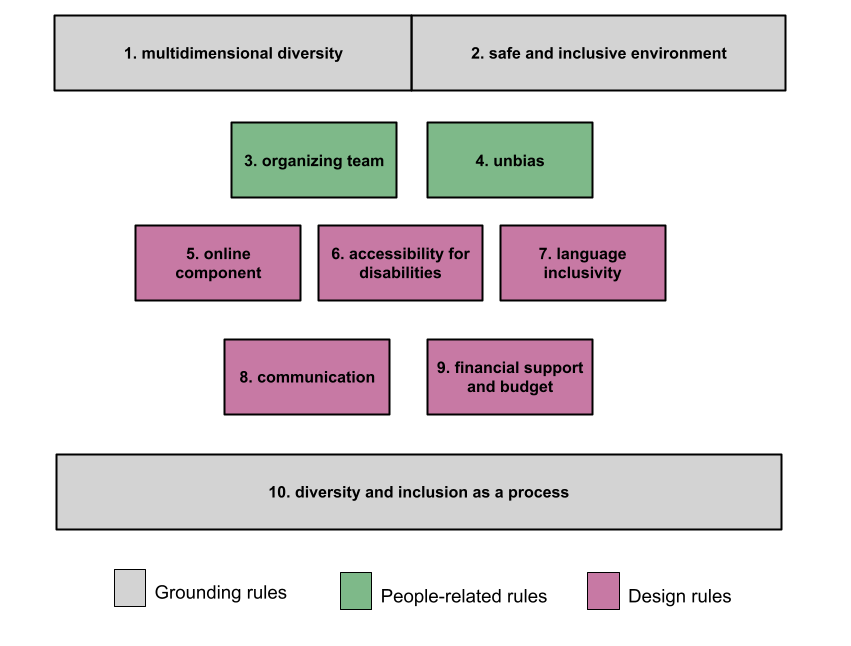
\includegraphics[width=\textwidth]{figs/10_rules_diversity.png}}{
%sara: suggestion for alt text:
Diagram of how the 10 rules are organized into three groups: grounding rules (rules 1, 2, and 10), people-related rules (rules 3 and 4), and design rules (rules 5 to 9). The diagram has five rows. Each line contains rectangular boxes with the rule number and a short title for each rule. Each rule box is colored based on their group (grounding rules are grey, people-related rules are green and design rules are pink). First row is for the grounding rules 1. Multidimensional diversity and 2. Safe and inclusive environment in grey boxes. Second row is for people-related rules 3. Organizing team and 4. Unbias in green boxes. Third row is for the design rules 5. Online component, 6. Accessibility for disabilities, 7. Language inclusivity in pink boxes. The fourth row is for the design rules 8. Communication and 9. Financial support and budget in pink boxes. The last row is for the grounding rule 10. Diversity and inclusion as a process in grey boxes.
}
\caption{Diagram of the rules organized in three groups: grounding rules (rules 1, 2, and 10), people-related rules (rules 3 and 4), and design rules (rules 5 to 9).}
\label{fig:diagram}
\end{figure}

% Dorothea: I like the intro as it is now, and I don't think the following paragraph is necessary.
% Rocío: I'm leaving this out now and seeing if we don't need this description of communities
%% Rocío: Main message of the paragraph: We do this for communities and people. What do we mean by communities and why are they important? (Why are they important may need some text)
%This article suggests rules to pivot traditional conferences towards diversity and inclusion, and strive to build more inclusive and welcoming communities. 
%Some scholarly or technological communities are formally structured as learned societies (e.g. the International Geographical Union or the Royal Statistical Society), others are composed by networks of less formal local groups (e.g. R User Groups or Python User Groups), and others may not have any established structure. 
%For the latter, conferences may play even a bigger role in shaping the community, since there is no other organization or institution to gather the community members. 

% keeping references:
%   However, conferences can become discriminating spaces, in which members of some specific privileged groups reproduce the systematic inequalities that occur in academia and society \cite{arendDisparityConferenceRegistration2019, timperleyHeMoanaPukepuke2020, gewinWhatScientistsShould2019, brownAbleismAcademiaWhere2018}.
% Liz adding reference marks2021meeting

\section{Embrace all dimensions of diversity}
\label{rule_diversity}

% Rocío: Main idea: what is diversity and why does it matter? (inequalities)
Diversity encompasses multiple dimensions: age, physical ability, career stage, gender, gender identity, geographic origin, language, neurodiversity, race, religion, sexual orientation, and socioeconomic background, to name a few\fede{we could substantiate this with one or two refs?}.
Human diversity should be celebrated and respected in every way. Nonetheless, we live in a world with implicit hierarchies along these axes. Some statuses (e.g., cisgender, white, male, from the United States or Western Europe) hold the privilege of being the defaults centered around which all systems--including conferences--are consciously and unconsciously built.  
While no isolated initiative can change reality by itself, building a more diverse and inclusive conference starts by recognizing that these inequalities have systematically excluded whole groups of people from academia and scientific and professional circles \cite{timperleyHeMoanaPukepuke2020}. 

% Rocío: more effort towards including the more excluded
Recognizing our privileges--unearned advantages given by society to some people but not all--particularly in our field and in our scientific or professional community, will help identify which subgroups have been the most excluded or discriminated against. 
These are the groups we need to make more effort to include. \fede{General thought: I like the way we say WE and YOU. I still think I saw most such 10SR papers speak to the readers addressing them with the roles. Which would be "Organizers", "Attendees". Just my 2 cents as avid reader of 10SR papers ;)}
Investing more effort in the most excluded groups does not mean neglecting the others, but it will guide the vision of diversity for your conference--and your strategies to achieve it.
Will a more diverse conference translate into a gender distribution of your speakers that is representative of the general population? 
Would it be the presence of racialized people --especially Black people-- among the head organizers, speakers, and attendees? 
Would it be having LGBTQIA+ friendly-spaces or community participation from key geographic regions?
%"The answer to these questions depend on your field, region or community.
Intersectionality, or the complex, cumulative way in which the effects of multiple forms of discrimination combine or intersect, should be taken into account. 


%batool: There are a few references which define privilege and might be good to add here including: Friedman, S., O’Brien, D., & McDonald, I. (2021). Deflecting Privilege: Class Identity and the Intergenerational Self. Sociology, 55(4), 716–733. https://doi.org/10.1177/0038038520982225
%batool: Another one is: Crevani, L. (2019). Privilege in place: How organisational practices contribute to meshing privilege in place. Scandinavian Journal of Management, 35(2). https://doi.org/10.1016/j.scaman.2018.09.002
%batool: please note that I didn't read both entire papers I mentioned above.
%sara: reference for privilege: McIntosh, Peggy. "White privilege: Unpacking the invisible knapsack." (1988).
% Rocío: I feel like we don't need to cite any reference about privilege the way it is now. But feel free to disagree.
%Dorothea: I agree with Rocío. citations for priviledge feel like citation for gravity...the current wording is not saying "there is priviledge, as shown by xyz. it says there is priviledge and we need to see where it is particularly strong in our field.


\section{Create a safe and welcoming environment}
\label{rule_inclusion}

% Rocío: main idea: Inclusion for everyone
While it is essential to improve representation towards some of the most visible dimensions of human diversity, such as race, gender, and country of origin, building a truly inclusive environment means taking care of all the other aspects of diversity as well. 
Having consideration of religious practices, setting specific accommodations for breastfeeding and child care, having LGBTQIA+-friendly spaces, creating community-only spaces, and acknowledging that gender is not binary are just some examples of decisions that can make inclusion real.
Importantly, you can take active steps in creating a more welcoming environment without requiring anyone to disclose personal information.

% Rocío: main idea: Code of conduct for a safe place
Adopting a code of conduct and gathering a team to enforce it are key aspects in creating a safe environment during a conference \cite{favaroYourScienceConference2016}.
%Dorothea: it is not a document, right? The document will not keep the community safe. Maybe say "a set of rules" in case someone doesn't know what a code of conduct is?
The code of conduct is a document meant to keep the community safe and should state clearly the unacceptable behaviors, the consequences for engaging in such behavior, and the way to report violations \cite{auroraHowRespondCode2019}. 
The code of conduct team must receive training on how to receive reports, respond to incidents, communicate their responses, and organize accordingly. 
Assembling a diverse code of conduct team will be more understanding of power dynamics and sensitive to discrimination and harassment issues. 
There are also disciplinary cultures and geographical considerations that may need to be considered when developing and communicating the code of conduct. 
We strongly recommend reading `How to Respond to Code of Conduct Reports' \cite{auroraHowRespondCode2019} as an excellent starting point for the code of conduct teamwork.
% Rocío: two of these sentences, diverse CoC team, and communication of CoC, may belong to rules organizing team and communication, respectively. 

% Rocío: Could have a paragraph about active bystandership—Andrea
%ast: tiny: check CoC capitalization (LA)

\section{Have an inclusive and diverse organizing team}
\label{rule_organizing_team}

% Rocío: Idea of this paragraph: build a diverse team
A genuinely inclusive conference can only be organized by an inclusive and diverse organizing team, in charge of the conference decision-making.
Organizers should build a team with people from different regions, genders, races and ethnicities, socioeconomic statuses, and other aspects of diversity. 
Go beyond balancing all genders in this effort and pay special attention to to intersectional diversity (see \textbf{Rule \ref{rule_diversity}}). 
To ensure a deep understanding and smooth communication with different diverse groups, it is essential to create a representative working group that functions as a snapshot of the general population.
If you already have an organizing team, check for gaps in its composition. 

% Rocío: Idea of this paragraph: real inclusion when having diverse members
Gathering a diverse team will only work if there is real inclusion. 
People with disabilities often say: `Nothing about us without us'; the same holds for other dimensions of diversity. 
This means that the actual life experiences, expertise, and insights from people in marginalized groups cannot be replaced by good intentions from people outside these groups \cite{costanzachockDesign2020}.
People who have experience with exclusion have the social and technical expertise about removing barriers to inclusion.
A truly inclusive and welcoming space is one in which everyone in the team is invited to be part of the solution.
However, do not expect people from minoritized groups to only work on these solutions, and respect their interests in other areas of the organization. 

% Rocío: Idea of this paragraph: positive outcomes of having a diverse team - keeping it general at least
Creating and maintaining such a team and space may seem more challenging than working in homogeneous teams--especially when you are not used to them--but the positive outcomes are worthwhile. 
Having diverse people in decision-making positions will affect positively all the other aspects of your conference because all the processes will benefit from their input, expertise, and distinct perspectives \cite{hongGroupsDiverseProblem2004}. 
In addition, a diverse team plays an important role at creating a welcoming space because representation--seeing people with similar life experiences occupy public spaces, positions of power, and breaking negative stereotypes--is one of the best ways to create a sense of belonging for everyone participating in the conference (see \textbf{Rule \ref{rule_inclusion}}). 


% Rocío: Idea of this paragraph: tips to make a diverse and inclusive team work.
The following advice should apply to any kind of team, but is specially relevant when working with people from marginalized groups. 
Do not expect self-nomination and voting to work as mechanisms to counteract systemic inequalities. Instead, nominate directly and offer leading positions, and let people from privileged groups step down.
Build an environment in which every person can express their position and give priority to people from systematically excluded groups.
Offer support and encouragement if you encounter cases of impostor syndrome. 
You can, for example, break the expectations about leadership as a lonely task and create smaller, co-led groups, where everyone finds their preferred tasks and gets to take leadership. 

% Rocío: Idea of this paragraph: take care of your team.
Most importantly, take care of your team. 
Having a diverse team and executing inclusive and accessible practices throughout the organizing period--it might be a year or two--may require a lot of effort. 
%Dorothea: I would remove the following sentence, I think we have made the point that it is worthwhile
The effort is worth it because it strengthens the event and the community making it truly welcoming for everyone. 
However, having a strong community as the only reward may be enough for those who are in more privileged positions. 
Some people and often the minoritized ones do not have institutional support to put time and effort into the organization tasks and do not have the luxury to commit to the organization for free; consider paying them as an item in your budget.  
In addition, tasks such as receiving and responding to code of conduct reports, can be emotionally intense work and should be additionally rewarded.
Prioritize your team's well-being. Check on them regularly and make sure everyone is comfortable. 
Be mindful of each particular context, be flexible with hours or commitments, and revise your budget (see \textbf{Rule \ref{rule_financial}}). 

% % Rocío: might go to the next rule
% Splitting the workload and responsibilities should not be done by putting care-taking labors--community building, meeting organization and note-taking, conversations with potential partners--on the hands of women and other minoritized groups, while people from privileged groups take the lead in stereotypical highly-valued tasks (see \textbf{Rule \ref{rule_unbias}}). Make work visible, discuss collectively what should be done (and why), divide and account work. Being transparent and sharing the information is key to make work visible and collective. %sara: this relates to make labor visible from DF, maybe we can cite them here too. %Rocío: sure.

%This is specially important for networking spaces, where receiving ideas, direct feedback, and spaces to co-lead from a wide variety of community members can be the key to organize meaningful sessions for all the conferences attendees. This gave a sense of variety and an appeal of "at least one networking session for everyone".  (Marcela)
%ast 17sep: i think we can talk here about planning neworking here, but also: the whole paragraph applies to team dynamics in general. Sara: maybe you can use this as we spoke relating team work here. And I think the working together part is not here but the following paragraph 
%sara: The last sentence in the paragraph sounds odd to me, but maybe I'm missing something. Andrea, I added a few sentences to the following paragraph regarding work dynamics
% Rocío: the rule is getting too long and, since this is focused on networking, I'd prefer it to go to a networking section.

\section{Consciously mitigate bias in your spotlight roles}
\label{rule_unbias}

%idea of paragraph 1: our lists are biased
When choosing or inviting people as keynote speakers, program committee, session chairs, and other spotlight roles, it is likely that there will not be much diversity in the first set of names. 
Many of our biased lists are products of the existing systems that have always privileged some groups of people \cite{dwyerNoticeWhoScience2021,swartzScienceValueDiversity2019,wongBuildDiversityScience2020,dignazioUnicornsJanitorsNinjas2020}. 
Rather than deter us, this implicit and systemic bias should encourage us to look further to find great people that are not routinely in the spotlight. 
Ensuring diversity in each of these roles needs to be a deliberate process. 
We need to go beyond our narrow and often limited networks to look for, reach out to, invite, encourage, and onboard these people until there is ample representation across the diversity spectrum and dimensions. 
\doro{The last sentence sounds odd. Maybe just: "until there is ample representation."}
Make sure that every selection committee--the committee looking for keynote speakers, the selection committee for abstracts, the prizes and award committees--are also diverse \cite{swartzScienceValueDiversity2019, wongBuildDiversityScience2020}, and ask them to be aware that everyone has implicit biases, to recognize them, and try to counteract them. 
An inclusive and diverse organizing team (\textbf{Rule \ref{rule_organizing_team}}) is already a great starting point to overcome this bias in other roles. The regional and local communities in your field are also good sources to tap into. 

% Rocío: main idea: unbias roles and give spotlight to the roles--and people who have contributed in roles--that are not stereotypically categorized as success
In academia and the industry, not only is the list of people considered in spotlight roles usually biased, but the spotlight roles themselves are.
Scientific publication and development of software, are often regarded with higher value than community building or teaching, which may be equally if not more challenging, less rewarded, and usually tackled by women, people of color, people with disabilities and from other minoritized groups \cite{cheng2020x+, burfordHomelinessMeantHaving2020}.
Defy the stereotypical criteria for success by acknowledging these community practices and the people behind them.
You can, for instance, give more space in your conference to talks about community building as an area of knowledge production, and reframe \doro{amend?}\fede{or, "promote a format for..."} the awards ceremony to acknowledge those who prepared accessible slides and presentations (see Rule \ref{rule_accessibility}), for being mindful of inclusiveness. \doro{Suggestion: "amend the awards ceremony to also acknowledge those who prepared accessible slides and presentations, contributed to community building or presented teaching materials"}
Finally, do not restrict people from marginalized groups or community-builders to talk or work only on issues related to diversity and inclusion; recognize their areas of expertise and interest and offer them space to showcase them. 

\section{Have a strong online component of the conference} 
\label{rule_online}

% Rocío: main idea of the paragraph: online conferences can open opportunities for inclusion
In-person interaction in conferences is priceless, but often this is true and possible only for the ones who can afford to attend. 
Barriers such as cost of registration, transport and accommodation, the logistics of long-distance travel, and discriminatory visa applications, are particularly true for conferences that usually take place in high-income countries \cite{arendDisparityConferenceRegistration2019,gewinWhatScientistsShould2019,jooKeepOnlineOption2021}. 
Online conferences are more inclusive because they do not require a visa or a big budget, and are more accessible to people who may be unable to travel because of health issues or family responsibilities \cite{salibaGettingGripsOnline2020}.
This means that online conferences will have a greater reach, not only in terms of participants but in terms of the tutors and presenters that can participate \cite{atkinsonJournalMedicine20202021, roosOnlineConferencesNew2020, jooKeepOnlineOption2021}.
The online format may also make it easier to be inclusive of geographic regions by encompassing several timezones in the week or easily deciding to rotate the favored timezone year to year, without depending on a conference central location. 

% Rocío: main idea of the paragraph: In the context of reopening, hybrid conferences may be a thing. They also need to be inclusive.
Within the context of the COVID-19 pandemic, many conferences embraced the online format; but at the time of writing, some are reverting to in-person, which risks going back to the barriers mentioned above.
Alternatively, a conference could have a hybrid format with an in-person and an online components that articulate well into a hybrid format that maximizes the experience of everyone attending your conference. This dual format could allow a group of people to interact face-to-face while providing many others the opportunity to participate remotely. 
The challenge and requirement for this kind of setting would be to make the online component as relevant as the in-person component and not just a "consolation prize" to the less privileged in the community \cite{ninerBetterWhomLeveling2021}.
%Needless to say, an online component is not inclusive \textit{per se} without taking many other precautions, and it does not eliminate the need to organize an inclusive in-person component. 
%For instance, to avoid favoring the same regions in every edition, we suggest rotating the location of the conference—if it is global, moving from one continent to another. 
% Rocío: Now I'm not sure if we need the last two sentences that I commented. 

% Rocío: main idea: Networking may seem the weakest part of online conference, but it doesn't have to be. 
% Rocío: I'm still doubting if this should be the 2nd paragraph, and I think that it needs some editing.
Networking and socializing have been mentioned as challenging aspects of online conferences, mostly because we are used to interactions at in-person social settings such as coffee or lunch breaks \cite{salibaGettingGripsOnline2020, roosOnlineConferencesNew2020}. 
However, in-person settings might not be comfortable or appealing to everyone for socializing; 
some of these spaces may be exclusionary (e.g. galas or dinner nights at expensive venues), and common place for code of conduct violations to occur \cite{auroraHowRespondCode2019}. 
On the other hand, there is evidence that virtual communication before face-to-face interaction can make people from minoritized groups feel more included, thus participate more (e.g. \cite{trianaDoesOrderFacetoFace2012, blackEngenderingBelongingThoughtful2020}). 
Organizers of online conferences should invest time in creating opportunities to meet and bond virtually, respecting people's limits, preferences, and remembering that `the usual' does not necessarily work for everyone, and that one single networking activity will never serve the whole community. 
It is worth trying new and varied activities that might work with subgroups of attendees.
Some ideas in this line are: offering the option of written chat only, instead of voice or video conversations, opening events with teamwork like trivia, offer some events that can be enjoyed passively like movies, yoga sessions, or art displays, where attendants can choose to just sit and enjoy without talking, or have a chat channel to comment on their experiences during the session.\fede{another activity: virtual city tours, I had it as a corollary activity for a summer school}


\section{Make the conference accessible to people with disabilities}
\label{rule_accessibility}


Conferences are among the least accessible spaces that people with disabilities may encounter \cite{priceAccessImaginedConstruction2009}. Even when conferences implement other inclusive practices, the participation of people with disabilities is often overlooked \cite{marks2021meeting}. This is one key aspect where having someone in the organizing team allows them to take part in the decisions from the beginning (see \textbf{Rule \ref{rule_organizing_team}}), as thinking about disability or simulating it are not substitutes for real-life experience \cite{costanzachockDesign2020}. Planning for accessibility requires time and early decision-making \cite{irishIncreasingParticipationUsing2020}. As other aspects of inclusion, dealing with accessibility at the last minute is the recipe for a disastrous conference. If you do not consider accessibility from the conference inception, it is highly likely you will be better off without trying to patch accessibility at the last minute. Key decisions in this respect are hard to correct. 
For in-person conferences, the venue should comply with common accessibility standards, such as being adequate for people who use wheelchairs, have signs in Braille, and a sound system compatible with hearing devices and live interpretation, just to name a few important features. In addition to this, the organizers should take care proactively of "invisible disabilities", for example, by providing quiet spaces for privacy and noise-free conversations, provide chairs in open spaces, and menus that include sugar-free, gluten-free, and alcohol-free options.

Regardless of the conference format, all platforms (website, chat, conference administration tools) and images used for the communication strategy of the conference should be screen-reader friendly and keyboard accessible, and have alternative text. Any videos should have captions and a transcript. 

The organizing team should provide accessibility guidelines for slides and presentations, encourage their use, and be available for any questions presenters and attendees may have. Slide decks should be made available beforehand, either in webpages or available for download to ensure that everybody can follow their content during the presentations. 

Accessibility practices should also include social events and networking, and include activities that do not restrict participation based on body type or ability. Importantly, all these accessibility practices are inclusive not only for people with disabilities but to everyone %ast: refs here.
For instance, captions are helpful for non-native speakers, having the material available for download helps attendees with low bandwidth connection, etc. Accessibility efforts should be explicitly displayed in the official communications of the conference (see \textbf{Rule \ref{rule_communication}}). 




\section{Don't let language restrict high-quality participation}
\label{rule_language}

% Rocío: main idea: English as the only language makes some people privileged and is a barrier for others
In international conferences, the linguistic diversity of conference participants is often overlooked. 
English is usually the official and sole language for submissions, presentations, tutorials, workshops, conference platforms, webpage, and official communications. 
While English is the primary language in scientific communication and one official language makes it conducive to communicate widely, this makes being a native English speaker a privilege.
Non-native English speakers could miss opportunities to attend or actively participate in conferences (e.g. asking questions or participating in discussions),
and conferences may miss innovative contributions.

% Rocío: main idea: make conferences more linguistically inclusive
Providing a welcoming and diverse environment by encouraging the full participation of non-native English speakers is critical (Rule 2). 
Advertising the conference in several languages and considering having non-English workshops and presentations to help overcome this barrier. 
Allow the audience to ask questions in their native language and invite others to help translate it; conversely, if the presenter is not comfortable with questions in English, encourage people in the audience to help by rephrasing their questions or try to translate them; after all, the community should be supportive. 

% Rocío: we could eventually cite https://conferenceinference.wordpress.com/2020/11/30/when-language-is-not-a-barrier-a-tale-fr[…]istically-inclusive-conference-toma-pustelnikovaite/

% Not citing ninerBetterWhomLeveling2021 anymore for now.

%ast: I think ome ideas of the first and second paragraphs can be joined because some parts are in both (intimidation, the importance of not missing opportunities) and maybe some practical tips can be made? Do we add an invitation to "bear" with subtitles and other languages to the English monolingual audience? an invitation to be respectful of "bad English", from submissions to presentations? 
%in person: live interpretation is doable. online: translated captions, pre-recorded talks, english trancripts

\section{Express the welcoming spirit in your communication strategy}
\label{rule_communication}

%Rocío: Main idea: Include people in your communication 
Your communication strategy should reflect the spirit of the conference and be inclusive by design. 
As you design the promotion plan, actively reach out and promote the conference to people who have been systematically excluded. 
If part of the community has been historically discriminated against, emphasize that they are particularly welcome in this event and that the organization will make it a safe and inclusive environment. This could be done through publishing the diversity statement (e.g., https://user2021.r-project.org/about/diversitystatement/), the code of conduct, and accessibility guidelines and advertising financial support, or other creative ways that show that everyone is seen, respected, and welcome (Fig. MARMOTS).
Also, try to advertise the conference in multiple languages (\textbf{Rule \ref{rule_language}}) and multiple platforms (e.g. Twitter, Facebook, LinkedIn, conference website, mailing lists)--
part of your community may use a different platform than the ones who regularly attend the conference. 
With proactive inclusive communication strategies, potential attendees will be assured that this is their space and community too (e.g. having accessibility guidelines on your website sends a welcoming message to people with disabilities), without the emotional labor of contacting the organizers and be public about your commitment to equity and inclusion.

%Rocío: Main idea: Use inclusive language
Inclusive language--language free from words, phrases or tones that reflect prejudiced or discriminatory views of particular people or groups--should be used in all communications \cite{hallDesigningDiversityInclusion2019}.
Make the effort to teach yourself the vocabulary and the best ways to communicate to account for every culture and situation. 
Do not expect minoritized people to teach you--it's not their role--and accept feedback without being offended.

% % Rocío: not sure if this belongs to the rule—Andrea make a convincing case :-P
% As we mentioned previously, conference attendees should have ample opportunities to network with each other. However, having a diverse offer of networking opportunities that can appeal to people with different backgrounds, accessibility needs, and preferences can be challenging, especially if you have the mindset of organizing each activity for the complete pool of attendants. If you think of smaller activities that can reach specific groups, preferably co-led by community leaders, these sessions can be more productive successful, and inclusive than trying to organize one single activity that can please the whole community (\textbf{Rule \ref{rule_unbias}}). Some examples are the newbies sessions for first-timers, mixers lead by specific subgroups or communities, or leisure activities that reunite subgroups with the same interests: arts, exercise, sports, movies, etc.
%Adithi had said: "Assist newbies of the conference navigate through the conference as they might feel overwhelmed attending a conference." but i see batool included newbies here :) 

% Yani: We need to work a little more here, perhaps with some examples.
% Rocío: could add some ideas from here 
% https://www.science.org.au/files/userfiles/support/emcr/documents/one-page-summary-emcr-improving-diversity-web.pdf
% Batool: I will work on this rule to include more details by 25th of Sept 
% ast: Thanks Batool! i added a couple of comments. 

\section{Allocate adequate financial resources to support your conference goals}
\label{rule_financial}

% Rocío: main idea: Budgets are limited and need to choose priorities.
Conference budgets are usually limited and rely mostly on sponsorship and attendance fees. 
While some expenses might be more or less fixed, % Rocío: can we give examples?
% Dorothea: this depends so much on the conference type. I wanted to write "venue"but this is not true of course, so I don't know what to add. 
allocation of resources has to be intentional to support the goals of the conference towards inclusion. 
It is important to estimate the costs for these inclusive practices and define your priorities in advance, like paying the organizing team, necessary training (e.g. code of conduct), and accessibility practices (e.g. captions). 
Aditional support for attendees should also be considered in the budget: child care support, transportation fees, visa-related support (if in-person), internet connection services (for the virtual component). 
Consider that an online conference might reduce organization costs (e.g. no rental costs for a physical venue), allowing to redirect the money towards other inclusive priorities. 
Instead of depending on registration fees, ask sponsors to support specific items in your inclusion expenses.
%Dorothea: I slightly disagree with that one. Maybe just leave the first part out?

% Rocío: main idea: help take the burden out of participants for more inclusive participation
Registration costs are one of the largest barriers for conference attendance, and, if we are aiming for inclusiveness and representation, the socioeconomic context of participants, their country of origin, and their career status should be taken into account when determining the registration rates \cite{sarabipourChangingScientificMeetings2021, andalibPostdocQueueLabour2018, kaplanPostdocNot2012}.
(see https://spcanelon.github.io/useR2021-cost-conversion-tool/ for an example of conversion rates based on country of origin and career status). 
In general, people should have the option to locate themselves in a category they consider affordable, even with the possibility of a `pay what you can' approach. 
Resources permitting, you can aim to have a conference with no registration costs, but bear in mind that free events have a lower attendance rate than events with registration costs \cite{eventbrite_ultimate_2017}. 
Offering fee waivers to attendees is also a good option, but even then, other costs can be prohibitive. 
Scholarships or grants to attend the conference is a common way to boost participation from people from marginalized groups, and conferences usually ask for cover letters or applications from them. 
These programs are important for in-person participation to support travel and lodging expenses. 
For online conferences, granting fee waivers or support for hidden costs like internet connection is easier and cheaper. 
Lower costs for attendance and offering financial support instead of prestigious grants--that could look good in a CV--may reduce the number of people applying for them and allow you to help all applicants. 
Applying for loans, grants, and scholarships might be an emotionally demanding task, so if this scenario is likely, simplify the process of asking for financial support. 
%Dorothea: I understand what we want to say, but there is a slight contradiction between "reduce the prestige so that less people apply and we can help everyone and reduce the barriers so that more people apply"

% Rocío: Let's keep this in mind for the 10th rule or conclusion
% While some of these items are being implemented recently, others can encounter a certain degree of resistance, such as paying the organizing team. Don't be afraid to innovate and resist the institutional inertia. "We have never payed for this, and this has always been like that" will not take the conference towards structural change.
% %ast should we talk about the pandemic? something like: 
% With the COVID-19 pandemic and the shift to online (or hybrid) events, some expenses disappeared, leaving space for rearrangements in this sense.
% Depending on registration fees to support large budget items is not at all desirable, instead sponsors can be asked to support specific items in this list.


\section{Diversity and inclusion are processes}
\label{rule_process}

% Rocío: main idea: we're not changing everything at the beginning, the conference will not be perfectly inclusive
Do not expect the conference to be perfect. 
Resources, both in time and money, are always limited. 
Most importantly, there are systemic discrimination issues at higher levels (e.g. society, academia) that one conference cannot change. 
There will be resistance, but your courage to make changes will be a step towards a more diverse and inclusive community, and can have a huge impact in the lives and careers of often excluded and minoritized people.

% Rocío: main idea: be part of the process
Diversity and inclusion will be the norm in the long-term, if we see conferences as part of the structural change. 
After the conference is over, assess whether equity and inclusion goals were met during the meeting. 
This can be done internally within the organizing team and taking into account the attendees' point of view. 
Identify the things that worked towards your inclusion goals, and try to understand what went wrong and how people were excluded.
Importantly, make sure to share the information with future organizers so that they can use it as a starting point and keep working to improve inclusion in the next edition of the conference. 

% For many people working with diversity, one typical aim is institutionalizing diversity (Ahmed 2012). However, our aim is also a symptom that diversity and equity are not part of institutions, academic societies, and conferences. This rule is about the process of making diversity and inclusion possible and a complement to all the other rules. We believe we need to be accountable and we need to aim for permanence. Institutionality comes from a set of norms, values, and priorities and these determine who is allowed and how (Ahmed 2012). Our long-term goal is to set new norms, values, and priorities based on diversity. Organizing a diverse conference is part of the process of change. However, we cannot do everything at one conference or a few of them. It is important to have a bold vision and clear targets. Keep in mind that ideal actions are often not possible and resources are limited (both time of the organizing team and money. 

% If from the beginning we set diversity goals and actions for the conference, we can use that to be transparent and, later, accountable. Assess whether equity and inclusion goals were met during the meeting. This can be done internally within the organizing team and often also through the conference’s participants. Plan, balance and keep working to improve inclusion in the next edition of the conference. Try to propose permanent data collection to assess whether diversity and inclusion are actually being seen at the conference. We know that diversity and equity are not institutionalized, in fact, the system works to stop those who are changing the system (Ahmed 2019). We will find resistance, but diversity is a school. We also learn more about how people are being excluded, we learn that there are actions we can take to include more, and then, we can set higher goals on how to make inclusion possible.

\section*{Concluding remarks}

This article suggests rules to pivot traditional conferences towards diversity and inclusion, and strive to build more inclusive and welcoming communities. 
This set of ten rules stated here can be adapted depending on the conference format and settings.
We organized useR! during a global pandemic, and as a team, this was a challenging journey. 
We engaged in most of the practices mentioned here and learned others along the way. 

Organizing a conference and implementing inclusive practices are both learning experiences;
do not expect to achieve everything, set priorities and remember rule 10: diversity and inclusion are processes. 
If you are part of a stable meetings committee, you could encourage organizers to follow these rules. 
If more conferences and domains apply them, the process will get more streamlined, straightforward, and mainstream to adapt with minimal overhead.
And you will make a change towards healthier, stronger, and more inclusive communities.


\section*{Acknowledgments}
The authors of this piece would like to thank every single member of the organizing team of useR! 2021 [ \url{https://user2021.r-project.org/about/global-team/}] for their valuable contribution to an inclusive conference experience, and the R Foundation for trusting us with the organization of useR! 2021 and supporting us through the process. 


% \nolinenumbers

% % Either type in your references using
% % \begin{thebibliography}{}
% % \bibitem{}
% % Text
% % \end{thebibliography}
% %
% % or
% %
% % Compile your BiBTeX database using our plos2015.bst
\bibliography{community-science}
% % style file and paste the contents of your .bbl file
% % here. See http://journals.plos.org/plosone/s/latex for 
% % step-by-step instructions.
% % % 
% \begin{thebibliography}{10}

% \bibitem{bib1}
% Conant GC, Wolfe KH.
% \newblock {{T}urning a hobby into a job: how duplicated genes find new
%   functions}.
% \newblock Nat Rev Genet. 2008 Dec;9(12):938--950.

% \bibitem{bib2}
% Ohno S.
% \newblock Evolution by gene duplication.
% \newblock London: George Alien \& Unwin Ltd. Berlin, Heidelberg and New York:
%   Springer-Verlag.; 1970.

% \bibitem{bib3}
% Magwire MM, Bayer F, Webster CL, Cao C, Jiggins FM.
% \newblock {{S}uccessive increases in the resistance of {D}rosophila to viral
%   infection through a transposon insertion followed by a {D}uplication}.
% \newblock PLoS Genet. 2011 Oct;7(10):e1002337.

% \end{thebibliography}



\end{document}

